%%%%%%%%%%%%%%%%%%%%%%%%%%%%%%%%%%%%%%%%%
% Beamer Presentation
% LaTeX Template
% Version 1.0 (10/11/12)
%
% This template has been downloaded from:
% http://www.LaTeXTemplates.com
%
% License:
% CC BY-NC-SA 3.0 (http://creativecommons.org/licenses/by-nc-sa/3.0/)
%
%%%%%%%%%%%%%%%%%%%%%%%%%%%%%%%%%%%%%%%%%

%----------------------------------------------------------------------------------------
%	PACKAGES AND THEMES
%----------------------------------------------------------------------------------------

\documentclass[aspectratio=169,UTF8,11pt,t]{ctexbeamer}

\mode<presentation> {
	\usetheme{Madrid}
	\setbeamertemplate{footline}{} % To remove the footer line in all slides
	\setbeamertemplate{navigation symbols}{} % To remove the navigation symbols from the bottom of all slides
}

% User Defined Block %%%%%%%%%%%%%%%%%%%%%%%%%%%%%%%%%%%%%%%%%%%%%%%%%%%%%%%%
\usepackage{multirow}

\usepackage{setspace}
\definecolor{hanblue}{rgb}{0.27, 0.42, 0.81}
\definecolor{indiagreen}{rgb}{0.07, 0.53, 0.03}
\definecolor{indianred}{rgb}{0.8, 0.36, 0.36}
\definecolor{indianyellow}{rgb}{0.89, 0.66, 0.34}
\definecolor{babypink}{rgb}{0.96, 0.76, 0.76}
\definecolor{ao(english)}{rgb}{0.0, 0.5, 0.0}
%\setbeamerfont{block title}{size=\small}
%\setbeamerfont{block body}{size=\footnotesize}
\newenvironment<>{blueblock}[1]{%
	\setbeamercolor{block title}{fg=white,bg=hanblue}%
	\begin{block}#2{#1}}{\end{block}}
\newenvironment<>{greenblock}[1]{%
	\setstretch{1.3}\setbeamercolor{block title}{fg=white,bg=indiagreen}%
	\begin{block}#2{#1}}{\end{block}}
\newenvironment<>{redblock}[1]{%
	\setstretch{1.3}\setbeamercolor{block title}{fg=white,bg=indianred}%
	\begin{block}#2{#1}}{\end{block}}
\newenvironment<>{yellowblock}[1]{%
	\setstretch{1.3}\setbeamercolor{block title}{fg=white,bg=indianyellow}%
	\begin{block}#2{#1}}{\end{block}}

%----------------------------------------------------------------------------------------
%	PACKAGES
%----------------------------------------------------------------------------------------
\usepackage{graphicx} % Allows including images
%\usepackage{tikz}
%\usetikzlibrary{shapes.geometric, arrows}
\usepackage{listings}
\lstset{language=C++,
	columns=flexible,
	basicstyle=\small\ttfamily,                                      % 设定代码字体、大小
	%numbers=left,xleftmargin=2em,framexleftmargin=2em,                   % 在左侧显示行号
	%numberstyle=\color{darkgray},                                        % 设定行号格式
	keywordstyle=\color{blue},                                            % 设定关键字格式
	commentstyle=\color{ao(english)},                                     % 设置代码注释的格式
	stringstyle=\color{brown},                                            % 设置字符串格式
	%showstringspaces=false,                                              % 控制是否显示空格
	%frame=lines,                                                         % 控制外框
	breaklines,                                                           % 控制是否折行
	postbreak=\space,                                                     % 控制折行后显示的标识字符
	breakindent=5pt,                                                      % 控制折行后缩进数量
	emph={size\_t,array,deque,list,map,queue,set,stack,vector,string,pair,tuple,ifstream,ostream,Qt}, % 非内置类型
	emphstyle={\color{teal}},
	escapeinside={(*@}{@*)},
}


\title[\textit{Qt编程基础}]{Qt编程基础}

% \author
%     []
%     {}

\date{}

 \institute{中国地质大学(武汉)自动化学院}


\begin{document}
	
	\begin{frame}
		\titlepage % Print the title page as the first slide
	\end{frame}
	
	\begin{frame}{目录}
		\begin{center}
\begin{columns}[t]
\column{0.4\textwidth}
\tableofcontents[sections={1-2}]
\column{0.4\textwidth}
\tableofcontents[sections={3-4}]
\end{columns}
\end{center}
	\end{frame}

\begin{frame}[fragile]{~}
    \begin{yellowblock}{学习目标}
        \begin{enumerate}
            \item 掌握Qt开发环境的基本使用
            \item 了解基本的window界面框架
            \item 理解信号与槽机制
            \item 理解事件机制
            \item 理解模型/视图结构
            \item 学会简单动画绘图
        \end{enumerate}
    \end{yellowblock}
\end{frame}

\section{Qt简介}
\subsection{功能和应用}
\begin{frame}[fragile]{1~Qt简介}
\vspace{-3mm}
   \begin{block}{跨平台C++图形用户界面应用程序开发框架,\url{https://www.qt.io/}}
  \begin{itemize}
    \item 它既可以开发GUI程序,也可用于开发非GUI程序,比如控制台工具和服务器。
    \item Qt是面向对象的框架,使用元对象编译器生成扩展代码,易于扩展,允许组件编程。
  \end{itemize}
   \end{block}
\vspace{-2.3mm}
    \begin{columns}[T]
        \column{0.5\textwidth}
        \pause \centering 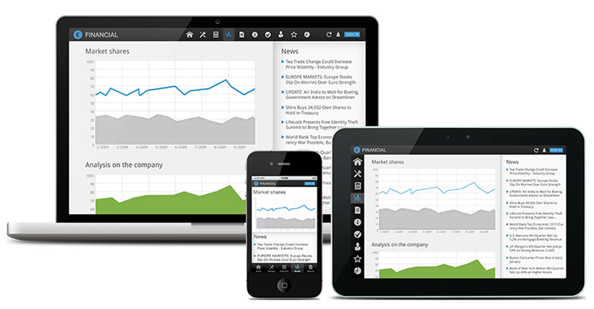
\includegraphics[width=0.66\textwidth]{fig/fig1} \vspace{-2.3mm}
   \begin{block}{跨平台}
 桌面:Windows, Linux, Mac; 移动:iOS, Android,WP; 嵌入式: QNX,VxWorks
  \end{block}
  \column{0.45\textwidth}
   \pause
 \centering 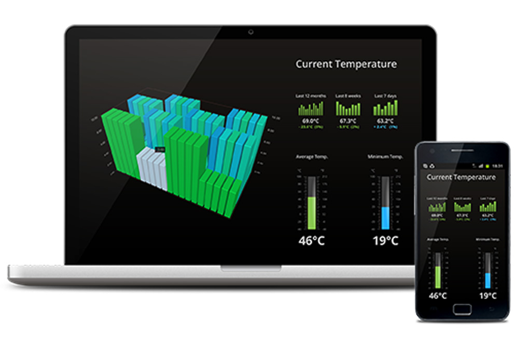
\includegraphics[width=0.58\textwidth]{fig/fig2}\vspace{-2.3mm}
   \begin{block}{集成开发平台}
 Design, Code, Debug \& Deploy Quickly\\
 ~~
  \end{block}
  \end{columns}
  \vspace{2mm}
\pause
\noindent \parbox{\textwidth}{应用:WPS、Skype、豆瓣电台、虾米音乐、VirtualBox、Opera、咪咕音乐、SMPlayer、VLC 多媒体
播放器、Google 地球、Adobe Photoshop Album、Texmaker、Opera、Qt Creator,\href{https://www.youtube.com/watch?v=gRYtG30yHxo&list=WL&index=10&t=6s}{\alert{Mercedes-Benz}},...}
\end{frame}

\subsection{版本和学习资料}
\begin{frame}[fragile]{1~Qt简介}
	\begin{block}{软件下载}
		\begin{description}
			\item[Qt版本] Qt 5: \url{https://www.qt.io/offline-installers}
		\end{description}
	\end{block}
	\pause
	\begin{block}{在线教程}
		\begin{itemize}
			\item Qt 学习之路:
\begin{itemize}
  \item \url{https://www.w3cschool.cn/learnroadqt/}
  \item \url{https://www.devbean.net/2012/08/qt-study-road-2-catelog/}
\end{itemize}
			\item Qt Documentation: \url{http://doc.qt.io/qt-5/gettingstarted.html}
			\item Qt examples:\url{http://doc.qt.io/qt-5/examples-widgets.html}
		\end{itemize}
	\end{block}	
\end{frame}

\section{Qt基础}
\subsection{信号和曹函数}
\begin{frame}[fragile]{2~Qt基础}
(1) 创建 Hello World Qt!
		{\begin{figure}
			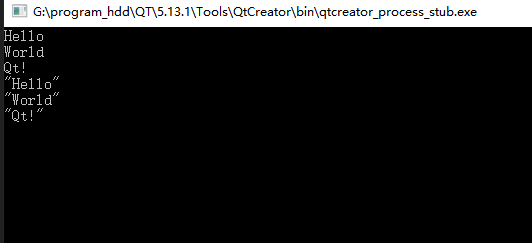
\includegraphics[width=0.6\textwidth]{fig/hello_word_qt.png}
		\end{figure}}
\end{frame}

\begin{frame}[fragile]{2~Qt基础}
	(2) 使用\alert{信号}与\alert{槽}机制实现简单的对象间通讯
	\begin{figure}
		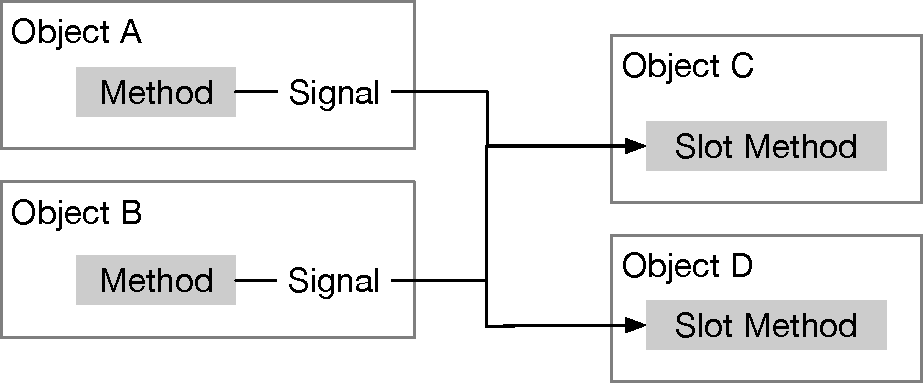
\includegraphics[width=0.45\textwidth]{fig/signals_slots.pdf}
	\end{figure}
			\pause
	\vspace{-7mm}
	\begin{columns}
		\column{0.48\textwidth}
		\begin{block}{信号 \texttt{signals}}
			\begin{itemize}
				\item 信号由对象发射
				\item 基类的信号被派生类继承
                \item 无实现,类似C++纯虚函数
			\end{itemize}
		\end{block}


		\column{0.48\textwidth}
				\begin{block}{槽 \texttt{slots}}
			\begin{itemize}
				\item 槽是普通的 C++ 成员函数
				\item 多个信号可以与其相关联
				\item 槽可以有参数,但参数不能有缺省值。
			\end{itemize}
		\end{block}

		\end{columns}
		\pause
				\begin{block}{信号-槽链接:connect(sender,  signal, receiver, slot)}
			\textbf{signal} 接口函数声明;
			\textbf{slot} 响应signal的实现;
			\textbf{sender} 发送消息的对象;
			\textbf{receiver} 接收消息的对象
		\end{block}
\end{frame}
	
	\begin{frame}{2~Qt基础}
	(2) 使用\alert{信号}与\alert{槽}机制实现简单的对象间通讯
		\begin{columns}
			\column{0.48\textwidth}
			\begin{block}{示例1-NewsPaper}
				\begin{figure}
					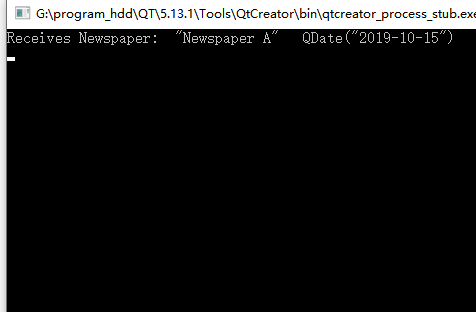
\includegraphics[width=1\textwidth]{fig/signal.png}
				\end{figure}
			\end{block}
			\pause
			\column{0.48\textwidth}
			\begin{block}{示例2-SliderSignals}
				\begin{figure}
					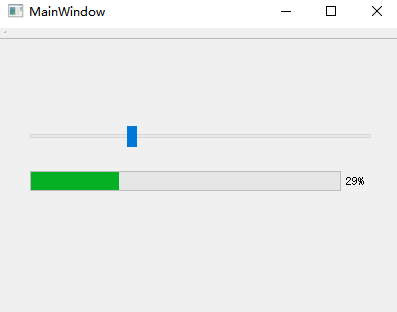
\includegraphics[width=0.83\textwidth]{fig/Slider.png}
				\end{figure}
			\end{block}
			\end{columns}
	\end{frame}
%	\begin{block}{}
%		\begin{description}
%			\item[public slots] 任何对象都可将信号与之相连接
%			\item[protected slots] 仅当前类及其子类可以将信号与之相连接
%			\item[private slots] 只有类自己可以将信号与之相连接
%		\end{description}
%	\end{block}
\subsection{GUI界面}
\begin{frame}[fragile]{2~Qt基础}
(3) 创建GUI界面
	\begin{figure}
		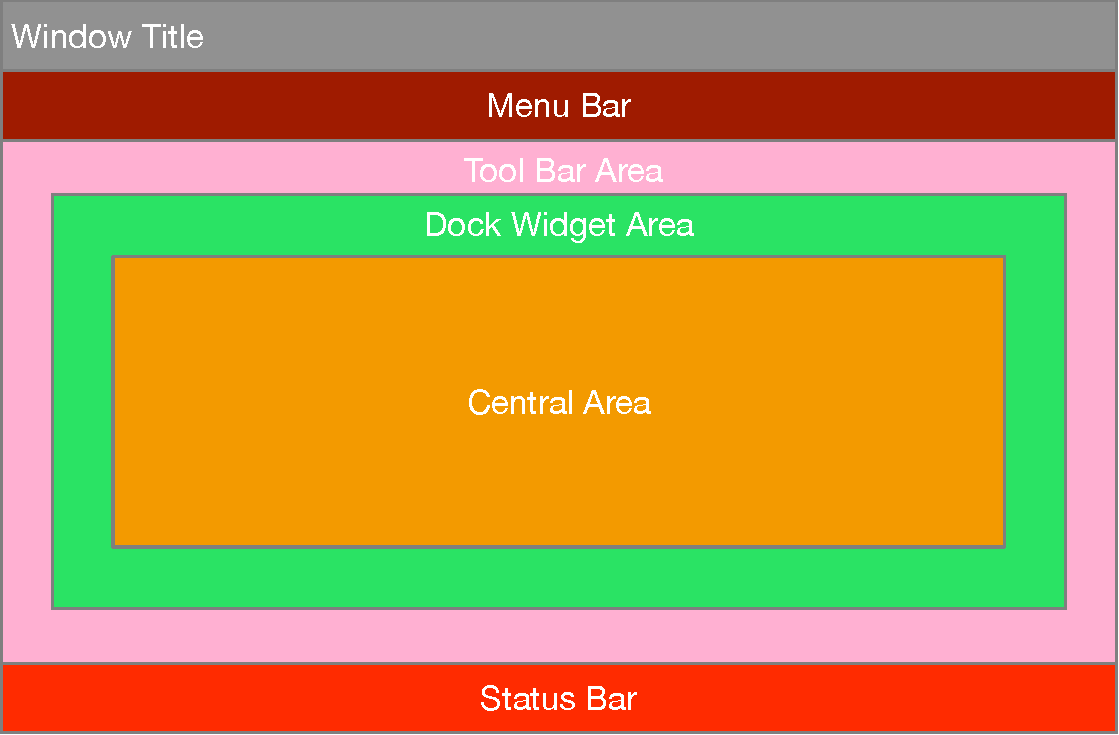
\includegraphics[width=0.6\textwidth]{fig/fig6}
	\end{figure}
\end{frame}

\begin{frame}[fragile]{2~Qt基础}
	(3) 创建GUI界面示例-Notepad
	\begin{figure}
		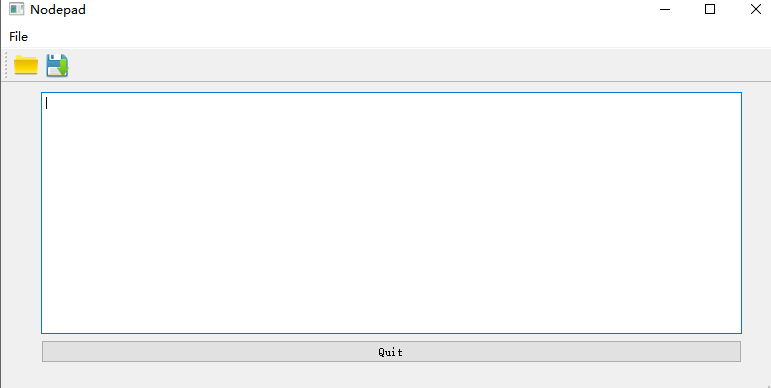
\includegraphics[width=0.7\textwidth]{fig/NotePad.png}
	\end{figure}
\end{frame}
\subsection{菜单和工具栏}
\begin{frame}{2~Qt基础}
	(4) 动作(action)-示例
			\begin{figure}
				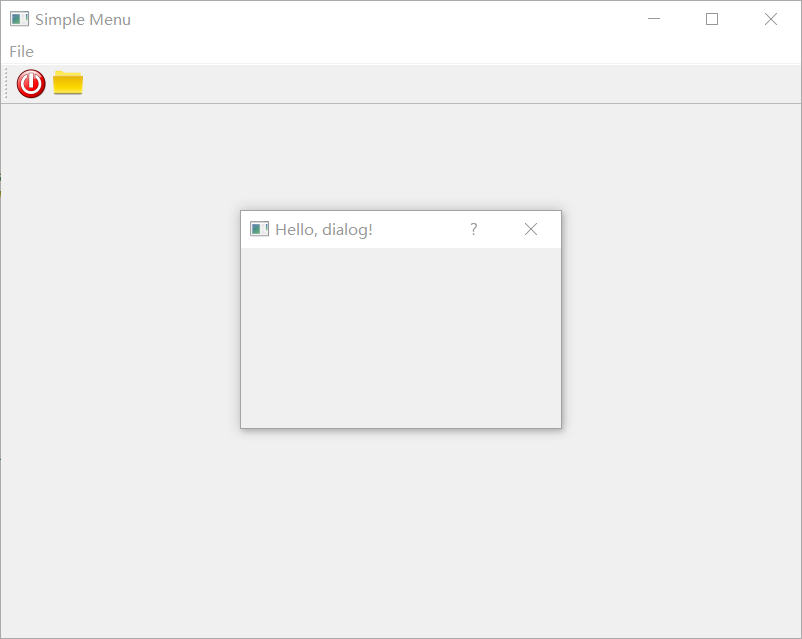
\includegraphics[width=0.5\textwidth]{fig/menu.png}
			\end{figure}
\end{frame}
\subsection{控件}
\begin{frame}{2~Qt基础}
(5) 使用设计模式添加控件示例-dialog
			\begin{figure}
				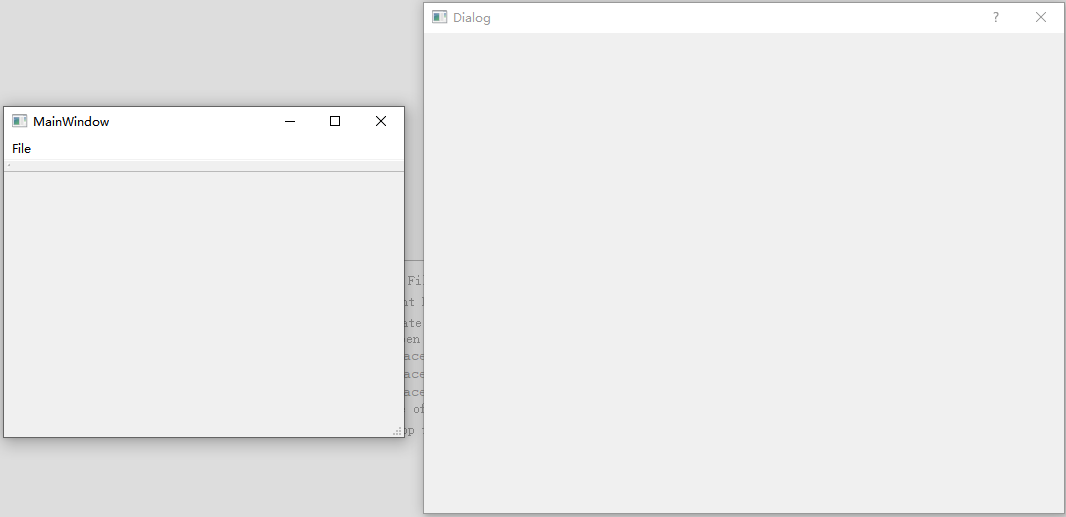
\includegraphics[width=0.7\textwidth]{fig/dialog.png}
			\end{figure}
\end{frame}
\subsection{布局}
\begin{frame}[fragile]{2~Qt基础}
	(6) 使用代码编辑UI控件布局
		\begin{figure}
			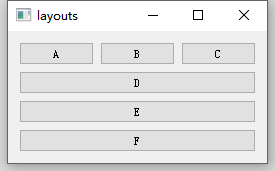
\includegraphics[width=0.45\textwidth]{fig/Layout.png}
		\end{figure}
	\end{frame}
\subsection{事件}
\begin{frame}{2~Qt基础}
		(7) 事件(event)
				\begin{figure}
					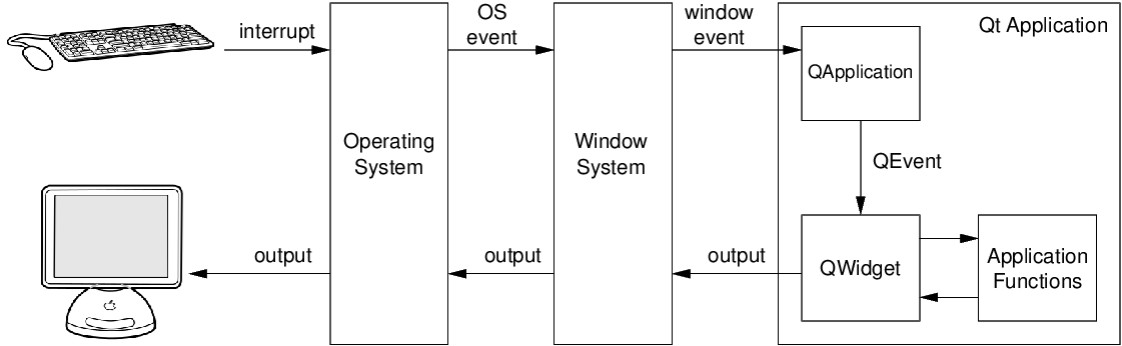
\includegraphics[width=0.8\textwidth]{fig/event_process.png}\\ \vspace{2mm}
\visible<2->{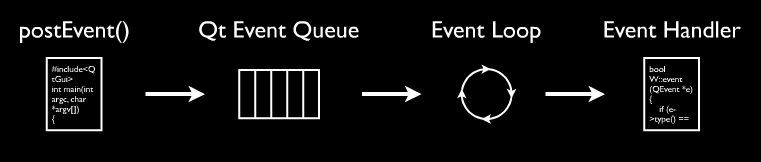
\includegraphics[width=0.8\textwidth]{fig/event_queue.png}}
				\end{figure}
	\end{frame}

\begin{frame}{2~Qt基础}
		(7) 事件(event)
				\begin{figure}
					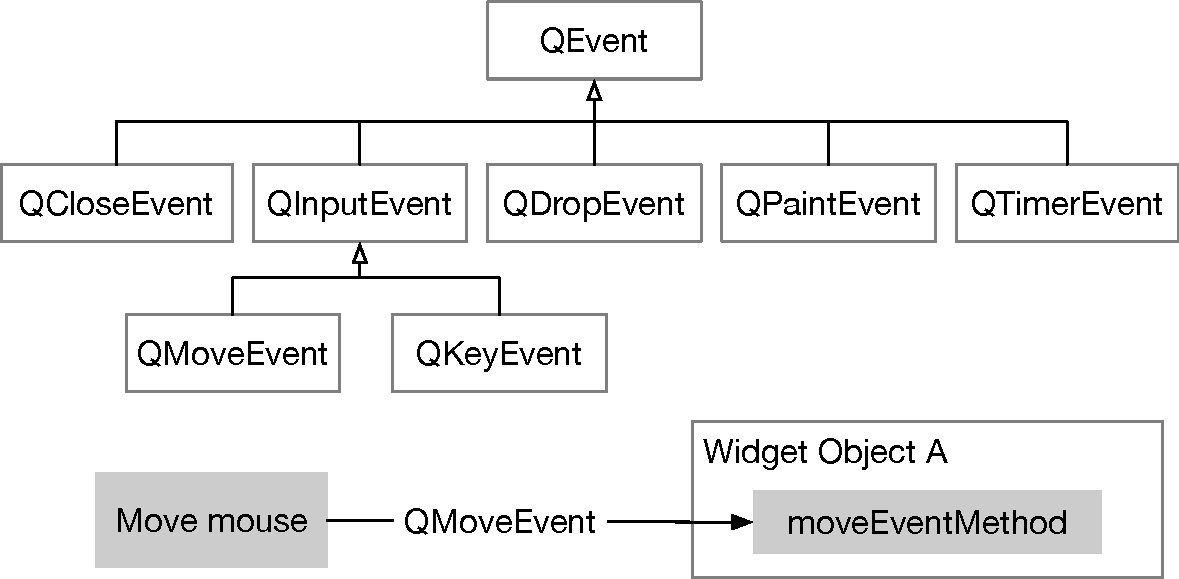
\includegraphics[width=0.75\textwidth]{fig/event.pdf}
				\end{figure}
	\end{frame}

\begin{frame}{2~Qt基础}
		(7) 事件(event)-示例
\begin{columns}
\column{0.6\textwidth}
				\begin{figure}
					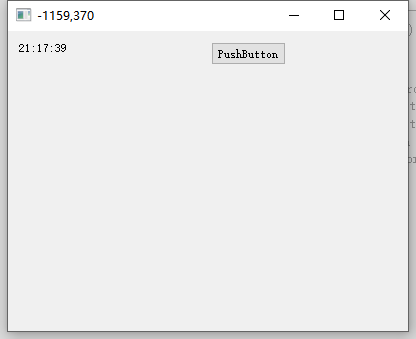
\includegraphics[width=0.8\textwidth]{fig/event.png}
				\end{figure}
\column{0.35\textwidth}
\begin{yellowblock}<2->{说明}
\begin{itemize}
 \item 事件不能等同于消息和槽机制
  \item 事件在组件层面上传播,而不是通过继承机制
  \item 通过事件过滤器接受相应事件或继续转发事件
\end{itemize}
\end{yellowblock}
\end{columns}
\end{frame}
\subsection{模型/视图结构}
\begin{frame}{2~Qt基础}
	(8) 模型/视图结构(Model/View)
			\begin{figure}
				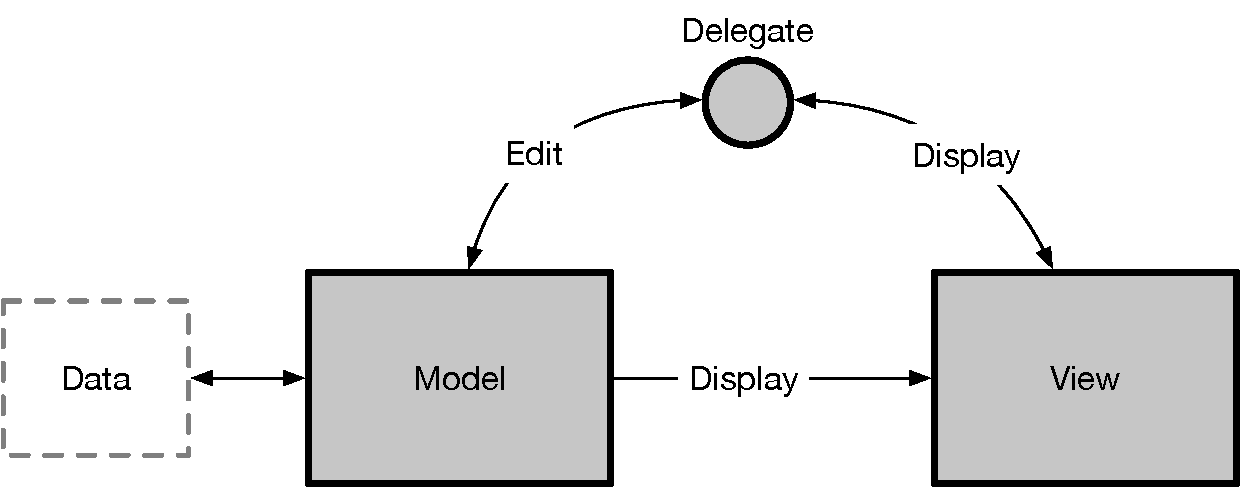
\includegraphics[width=0.7\textwidth]{fig/model_view.pdf}
			\end{figure}
\end{frame}
\begin{frame}{2~Qt基础}
	(8) 模型/视图结构(Model/View)-示例
\begin{center}
 \begin{tabular}{cc}
            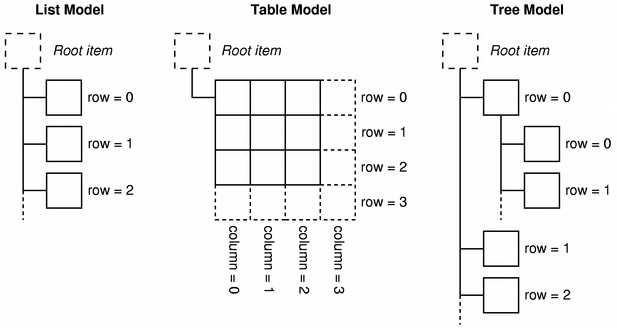
\includegraphics[width=0.55\textwidth]{fig/model_intro.png}&
			 \visible<2->{\includegraphics[width=0.4\textwidth]{fig/table_view.png}}
			\end{tabular}
\end{center}			
\end{frame}


\subsection{画图}

\begin{frame}[fragile]{2~Qt基础}
	(9) 画图(Painting)
 \begin{center}
       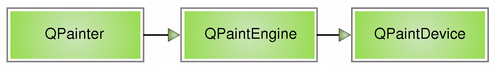
\includegraphics[width=0.7\textwidth]{fig/paintsystem-core.png}
    \end{center}
    \begin{itemize}
      \item QPainter(画笔)用来执行绘制的操作;
      \item QPaintDevice(画布)是一个二维空间的抽象,允许QPainter在其上面进行绘制;
      \item QPaintEngine提供了QPainter在不同的设备上进行绘制的统一的接口。
    \end{itemize}
\end{frame}

\begin{frame}[fragile]{2~Qt基础}
	(9) 画图(Painting)

\begin{columns}
    \column{0.33\textwidth}
    \begin{center}
       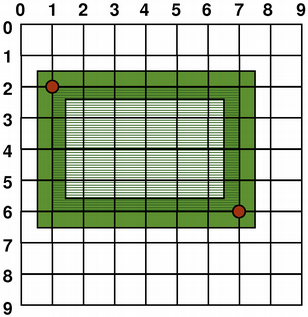
\includegraphics[width=0.7\textwidth]{fig/coordinatesystem-rect.png}\\
       坐标系
    \end{center}  
    \begin{lstlisting}[basicstyle=\scriptsize\ttfamily,   moreemph={QPainter,darkGreen}]
    QPainter painter(this);
    painter.setPen(Qt::darkGreen);
    //Using the (x  y  w  h) overload
    painter.drawRect(1, 2, 6, 4);
    \end{lstlisting}\vspace{-2mm}
    \column{0.33\textwidth}
    \begin{center}
    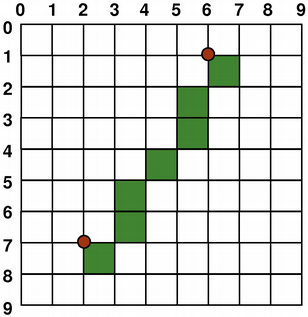
\includegraphics[width=0.7\textwidth]{fig/coordinatesystem-line-raster.png}
    \end{center} 
    \begin{lstlisting}[basicstyle=\scriptsize\ttfamily,moreemph={QPainter,darkGreen}]
    QPainter painter(this);

    painter.setPen(Qt::darkGreen);
    painter.drawLine(2, 7, 6, 1);
    \end{lstlisting}\vspace{-2mm}
    \column{0.33\textwidth}
    \begin{center}
    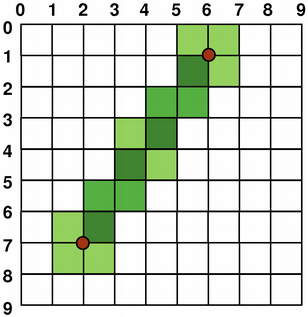
\includegraphics[width=0.7\textwidth]{fig/coordinatesystem-line-antialias.png}\\
    反走样
    \end{center} 
    \begin{lstlisting}[basicstyle=\scriptsize\ttfamily,moreemph={QPainter,darkGreen}]
    QPainter painter(this);
    painter.setRenderHint(
        QPainter::Antialiasing);
    painter.setPen(Qt::darkGreen);
    painter.drawLine(2, 7, 6, 1);
    \end{lstlisting}\vspace{-2mm}
\end{columns}
\end{frame}

\section{示例}
\subsection{时钟}
\begin{frame}{3~示例}
	示例一:时钟
	\begin{figure}
		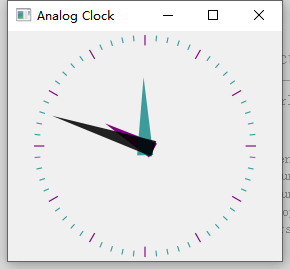
\includegraphics[width=0.4\textwidth]{fig/clock.png}
	\end{figure}
\end{frame}
\subsection{贪吃蛇}
\begin{frame}{3~示例}
	示例二:贪吃蛇
	\begin{figure}
		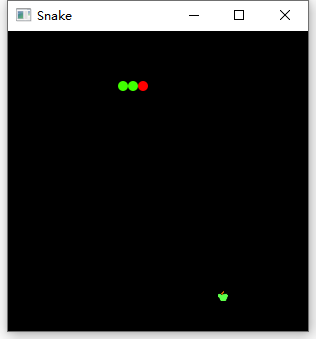
\includegraphics[width=0.4\textwidth]{fig/snake.png}
	\end{figure}
\end{frame}

\begin{frame}{第四次验收}
	仿照Windows系统的计算器软件,为教材第12.4节通用计算器设计界面,开发一款实用的计算器软件。
	\begin{figure}
		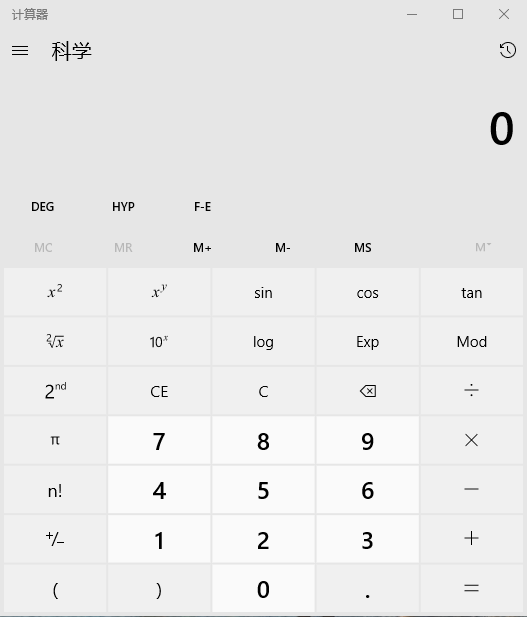
\includegraphics[width=0.35\textwidth]{fig/calculator.png}
	\end{figure}
\end{frame}

\begin{frame}{结课考核}
	学生成绩管理系统,按照实验指导书附录中课程设计报告模板要求撰写结课报告。
	
\end{frame}

\section{后记}
\subsection{C++程序设计总结}
\begin{frame}{4~后记}

\begin{columns}[T]
\column{0.18\textwidth}
\begin{block}{C++编程风格}
\begin{itemize}
\item 数据抽象
  \item 过程化
  \item 面向对象
  \item 泛型编程
\end{itemize}
\end{block}
\column{0.3\textwidth}
\begin{block}{C++知识层级}
\begin{itemize}
  \item 层级一:语法/语意
  \item 层级二:专家经验
  \item 层级三:底层机制
  \item 层级四:设计观念复用
\end{itemize}
\end{block}
\column{0.47\textwidth}
\vspace{2mm}

\begin{tabular}{@{}c@{~}c@{}}
 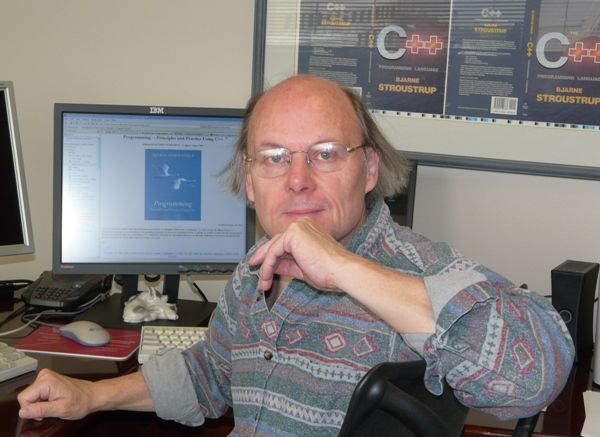
\includegraphics[width=0.55\textwidth]{fig/Bjarne.jpg} &  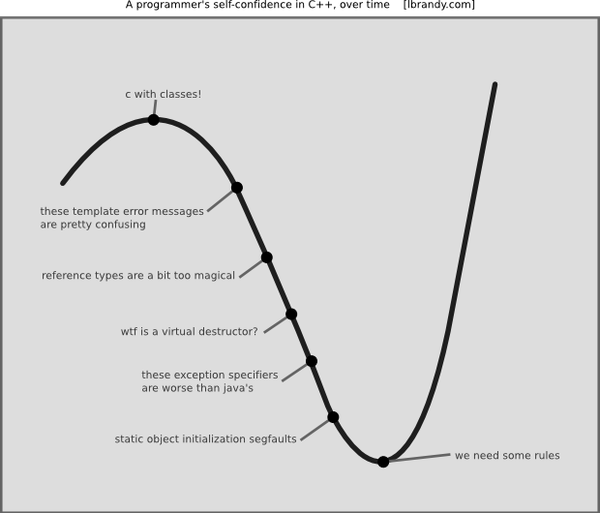
\includegraphics[width=0.48\textwidth]{fig/confidence.png}
\end{tabular}

\end{columns}
	
\begin{block}{网友的评价}
\begin{itemize}
  \item \alert{精通C++是一个艰巨的任务}。为什么C++比别的语言难学这么多?是因为C++他爹Bjarne Stroustrup说过的一句话“我特别讨厌语言的设计者把自己的喜好强加给用户”
C++能够自由的让你放弃某些部分,而别的语言会阻止你放弃某些部分。
  \item 谷歌工程师师对C++的掌握有两个级别:拥有C++的readability(可读性)认证;顾问级C++程序猿
  \item Never trust a programmer who says he knows C++
\end{itemize}
\end{block}
\end{frame}

\subsection{推荐书籍}
\begin{frame}{4~后记}
\begin{block}{推荐C++书籍}
\begin{itemize}
\item  层级一:语法/语意(C++)
\begin{enumerate}
  \item C++ Primer ( 中文版,侯俊杰 译) by Stanley B. Lippman
\end{enumerate}
\item 层级二:专家经验(C++/OOP)
\begin{enumerate}
  \item (More )Effective C++(中文版,侯俊杰 译), by Scott Meyers.
  \item (More )Exceptional C++ (中文版,侯俊杰 译), by Herb Sutter
  \item Effective Modern C++, by Scott Meyers
\end{enumerate}
\item 层级三:底层机制(C++ Object Model)
\begin{enumerate}
\item  Inside the C++ Object Model (深度探索C++物件模型,侯俊杰 译),by Stanley Lippman.
\end{enumerate}
\item 层级四:设计观念的复用(C++/Patterns)
\begin{enumerate}
\item Design Patterns:Elements of Reusable Object Oriented Software,
by Erich Gamma,Richard Helm,Ralph Johnson,and John Vlissides
\item Modern C++ Design: Generic Programming and Design Patterns Applied by Andrei Alexandrescu.
\end{enumerate}
\end{itemize}
\end{block}

\end{frame}
\subsection{编程能力}
\begin{frame}{4~后记}
\vspace{2cm}
\begin{center}
\begin{block}{编程能力:\alert{运用机器解决问题的能力}}
\begin{itemize}
  \item 深度:算法,数据结构,强化学习,模式识别、深度学习、智能优化
  \item 广度:操作系统,分布式系统,存储系统,游戏引擎、数据库、GPU, FPGA, AR/VR
\end{itemize}
\end{block}
\end{center}

\end{frame}

\subsection{寄语}
\begin{frame}{4~后记}
\vspace{3.5cm}
\begin{center}
{\huge \color{blue} AI之路漫漫其修远兮,吾将上下而求索}
\end{center}
\end{frame}
\end{document} 